\documentclass{article}
\usepackage{arxiv}
\usepackage[utf8]{inputenc} % allow utf-8 input
\usepackage[T1]{fontenc}    % use 8-bit T1 fonts
\usepackage{hyperref}       % hyperlinks
\usepackage{url}            % simple URL typesetting
\usepackage{booktabs}       % professional-quality tables
\usepackage{amsfonts}       % blackboard math symbols
\usepackage{nicefrac}       % compact symbols for 1/2, etc.
\usepackage{microtype}      % microtypography
\usepackage{amsmath}
\usepackage{graphicx}
\usepackage{array}
\usepackage{tabularx}

\title{Contact tracing and isolation reduces Covid-19 incidence in a structured agent-based model}

\author{
  Marcus Low \\
  Department of Computer Science \\
  University of Cape Town\\
  \texttt{LWXMAR013@MyUCT.ac.za} \\
  \and
  Nathan Geffen \\
  Centre for Social Science Research \\
  University of Cape Town\\
  \texttt{nathan.geffen@alumni.uct.ac.za}}

\date{\today}

\usepackage{listings}
\usepackage{color}

% For nicely formatting code
\lstset{frame=tb,
  language=Python,
  aboveskip=3mm,
  belowskip=3mm,
  showstringspaces=false,
  columns=flexible,
  basicstyle={\small\ttfamily},
  numbers=none,
  breaklines=true,
  breakatwhitespace=true,
  tabsize=3
}

\begin{document}

\maketitle

\begin{abstract}

Background: The World Health Organization has identified contact tracing and
isolation (CTI) as a key strategy to slow transmission of SARS-CoV-2. Structured
agent-based models (ABMs) provide a means to investigate the efficacy of such
strategies in heterogeneous populations and to explore the impact of factors
such as changes in test turnaround times (TaT).

Methods: We developed a structured ABM to simulate key SARS-CoV-2 transmission
and Covid-19 disease progression dynamics in populations of $10,000$ agents. We
ran $10 000$ simulations of each of three scenarios: (1) No CTI with a TaT of
two days, (2) CTI with a TaT of two days, and (3) CTI with a TaT of 8 days. We
conducted a secondary analysis in which TaT values were varied from 2 to 10. The
primary outcome for all analyses was mean total infections.

Results: CTI reduced the mean number of infections from 5,577 to 4,157 (a
relative reduction of 25.5\%) when TaT was held steady at 2 days. CTI with a TaT
of 8 days resulted in a mean of 5,163 infections (a relative reduction of 7.4\%
compared to no CTI and a TaT of 2 days). In the secondary analysis, every
additional day added to the TaT increased the total number of infections – with
the greatest increase in infections between four and five days, and the smallest
increase between nine and ten days.

Conclusions: In a structured ABM that simulates key dynamics of Covid-19
transmission and disease progression, CTI results in a substantial reduction in
the mean number of total infections. The benefit is greater with shorter TaT
times, but remained substantial even with TaTs of eight days. The results
suggest that CTI may play a critical role in reducing the size of outbreaks and
that TaTs should be kept as short as possible in order to maximise this benefit.

\end{abstract}

\keywords{SARS-CoV-2 \and Covid-19 \and Agent-based model \and Contact tracing}

\section{Introduction}

Many countries have implemented extended and far-reaching lockdowns in response
to the Coronavirus Disease 2019 (Covid-19) pandemic, often at significant
economic cost. A key question that has arisen in recent months is what
non-pharmaceutical interventions (NPIs) governments can implement in order to
exit such lockdowns as safely as possible.\cite{Han2020} Some potential NPIs
include promotion of hand-washing and other hygiene measures, promotion of or
legal requirement of mask-wearing in public, various physical distancing
regulations, border closures, school closures and contact tracing and isolation
(CTI).\cite{Flaxman2020}

The World Health Organization (WHO) has endorsed CTI as a key strategy to slow
transmission of SARS-CoV-2.\cite{WHO2020} CTI has been implemented in a wide
range of countries - maybe most notably in China, Singapore and South
Korea.\cite{Fisher2020, Lee2020, Lee2020b} One recent Lancet study concluded
that “each country should have an effective find, test, trace, isolate, and
support system in place”.\cite{Han2020} CTI involves tracing the recent contacts
of a person who tested positive for SARS-CoV-2 and isolating these contacts, and
in some cases also testing contacts. CTI is traditionally conducted by teams of
tracers, but can also be done through, or assisted by various mobile phone
applications. Since there are economic, human resource and opportunity costs
related to CTI, it is important to understand the effectiveness of such
programmes and the factors impacting their effectiveness.

A recent SARS-CoV-2 stochastic transmission modelling study found that
'minimising testing delay had the largest impact on reducing onward
transmissions' and suggested that, in their model at least, test turnaround
times (TaTs) of less than three days were required to get the effective
reproductive number under 1.\cite{Kretzschmar2020} A recent branch process
modelling study found that in most scenarios, highly effective contact tracing
and case isolation is enough to control a new SARS-CoV-2 outbreak within 3
months, but that 'the probability of control decreases with long delays from
symptom onset to isolation'.\cite{Hellewell2020} Such delays could for example
be due to long TaTs.

Structured agent-based models (ABMs) are a way to model the complex consequences
of interventions such as CTI on the transmission of SARS-CoV-2. By modelling at
the agent level, where each agent represents a person, such models better
account for heterogeneity within populations than is the case with compartmental
or population-level models that by definition model groups rather than
individuals. Though stochastic, neither of the two SARS-CoV-2 models cited above
are ABMs. In a recent review, four of seven models investigating CTI for the
control of earlier outbreaks of Severe Acute Respiratory Syndrome and/or
Middle-Eastern Respiratory Syndrome were agent-based models.\cite{Kwok2019}

The model we report on here is novel in that it (1) is a high performance ABM
calibrated to various Covid-19 parameters, (2) contains structure in the form of
households, school classes, workplaces, public transport and neighbourhood
blocks, and (3) allows for the modelling of interventions such as CTI and
variable TaTs within a structured and heterogeneous population.

\section{Methodology}

We developed a structured ABM, called ABM-Spaces, to simulate key dynamics of
the transmission and disease progression of SARS-CoV-2 in a closed population of
$10,000$ agents loosely based on the Masiphumelele township in Cape Town South
Africa. Each simulation was run for 270 time steps (days). Key elements of the
model world are as follows:

\begin{description}

\item[Agents:] Agents are given various attributes, including age, sex, and a
  variety of variables relating to disease states (exposed, infectious,
  symptomatic, recovered, dead, etc). Agents are newly created in each
  simulation, thus introducing variability in age structure, gender balance, and
  the number of initial infections.

\item[Settings:] Agents in the model are associated with settings
  (places). Based on research on tuberculosis transmission in Masiphumelele, the
  five types of settings in the model are households, school classes,
  workplaces, public transport (minibus taxis or train carriages) and blocks
  (collections of households).\cite{Andrews2014} All agents in the model belong
  to households. All school-age agents are placed into school classes. A
  percentage of working-age agents are placed into workplaces. Employed agents
  are more likely to take taxis. Each instance of the simulation stochastically
  creates new agents that are associated with newly constituted schools,
  households and workplaces based on parameters such as employment rate and the
  average size of school classes.

\item[Transmission:] Transmission of SARS-CoV-2 in the model occurs not directly
  from agent to agent, but from agent to setting to agent. On each time step in
  the model agents are exposed to the transmission risk of the various settings
  they are associated with. The setting and time step-specific risk of a setting
  is a product of the number of infectious agents in that setting on that time
  step and the inherent risk profile of the type of setting. This can be
  expressed as:

  \begin{equation*}
    r = n * ir
  \end{equation*}

  Where $r$ is the specific risk faced by a susceptible agent in a specific
  setting on a specific timestep, $n$ is the number of positive agents in a
  setting on a specific timestep and $ir$ is the inherent risk of the setting (a
  constant that is different for different types of setting).

  For each agent in each setting, on each timestep the model draws a random
  number $k$ from a uniform distribution of integers $1$ to $10,000$. If $k$ is less
  than $r$ transmission takes place. One variation on this is transmission in
  taxis where transmission only takes place if $k$ is less than the square route
  of $R$.

  The parameters for inherent risk ($ir$) associated with different settings
  were calibrated using two processes: First, setting-related risks were varied
  so as to reproduce published transmission patterns observed for TB in
  Masiphumalele.\cite{Andrews2014} Second, these risks were calibrated so as to
  produce epidemic simulations with $R_0$ values that fall within the range of
  $R_0$ estimates found in the Covid-19 literature.\cite{Hellewell2020}

  We calculated $R_0$ values using a numerical method that involves deriving
  $R_0$ from the equation $R = R_0 * S/N$ – where $S$ is the susceptible
  population and $N$ is the total population.\cite{Vynnycky2010} Since
  $R_t$ = 1 at the peak of the epidemic and the fraction susceptible at the peak
  of the epidemic is known for each simulation, $R_0$ can accordingly be solved
  numerically.

\item[Disease progression:] On the day an agent becomes infected with
  SARS-CoV-2, the model draws from a number of distributions and estimates of
  risk, based on the published Covid-19 literature,\cite{Verity2020, SACMC2020}
  to determine (1) whether the agent will become symptomatic and when, (2) when
  the agent will become infectious, (3) whether the agent will be tested and
  when, (4) whether the agent will stay home and when, (5) whether the agent
  will require hospitalisation and when, and (6) whether the agent will die and
  when. The model remains flexible regarding these values – for example to
  account for hospitals being full.

\item[Testing:] The model allows for false negative tests by taking into account
  published estimates of the variability of test sensitivity based on days since
  infection. \cite{Kucirka2020} We gave symptomatic agents a likelihood of 0.8
  of being tested – although the model can easily be run with other values for
  this and other variables. The only way for asymptomatic agents to be tested in
  the model is as part of contact tracing. The model allows for different TaT
  values to be used. TaT values observed in South Africa ranged from two to
  greater than 11. \cite{NICD2020}

\item[CTI:] The model can be run with or without CTI. In the default version of
  the model CTI involves testing 80\% of an agent’s household, school class or
  workplace contacts within two days of the agent testing positive. The test
  results for these tests become available a default of two days later (TaT = 2)
  whereupon the same process is repeated for all positive tests – with the
  modification that agents tested in the last 14 days will not be tested
  again. In CTI scenarios agents who test positive are isolated from all other
  agents and cannot further transmit the virus. 80\% of agents who are traced,
  but who do not test positive go into isolation, with the remaining 20\%
  isolating at home. The model can also be run so that a positive agent’s
  contacts are isolated, but not tested.

  Isolation refers to the movement of people with the infection being
  restricted, voluntarily or legally, while quarantine refers to the movement of
  people at risk of infection being restricted, voluntarily or legally. The work
  described here does not differentiate between these distinctions. We therefore
  use isolation to refer interchangeably to isolation or quarantine.

\end{description}

\subsection{Analysis}

To explore the impact of CTI we held TaT steady at two days and ran $10,000$
simulations without CTI and 10,000 simulations with CTI. We then ran an
additional 10,000 simulations with CTI and a TaT of eight days to test whether
CTI is still beneficial if there are significant testing delays. In these base
CTI scenarios the contacts of everyone who tests positive are tested. Since CTI
in the real world sometimes does not involve testing of contacts, we ran an
additional $10,000$ simulations of each of the CTI scenarios with the testing of
contacts removed.

As a secondary analysis to explore the impact of different testing delays, we
ran 10,000 simulations with CTI for each value of TaT from two to 11. This was
done with testing of contacts and repeated without testing of contacts.

\subsection{Programming}

Prototype versions of ABM-Spaces were developed in R, but the final version
presented here is coded in C++, which is dramatically faster than the R
version. The C++ code allows for thousands of simulations to be run in minutes
on standard consumer hardware and can easily be modified to explore different
research questions in a structured ABM environment. The ABM-Spaces source is
available under the GNU General Public License version 3.0. Our code and results
are available at \url{https://github.com/nathangeffen/ABM_CTI}.

\section{Results}\label{results}

CTI reduced the mean number of infections from $5,577$ to $4,157$, a relative
reduction of 25.5\%, when TaT was held steady at 2 days. CTI with a TaT of 8
days resulted in a mean number of $5,163 infections$, a relative reduction of 7.4\%
compared to no CTI and a TaT of 2 days. In CTI scenarios where contacts of
positive agents were not tested the reduction in the mean number of total
infections were more modest. CTI with a TaT of 2 days and no testing of contacts
resulted in a mean of 4,670 infections, while the same scenario with TaT
extended to 8 days resulted in 5,263 infections (relative reductions of 16.3\%
and 5.56\% respectively compared to no CTI).

\begin{table}[ht!]
  \centering
  \begin{tabular}{|l|c|c|}
    \hline
  Scenario & Mean total infections & Infections as fraction of no CTI \\ \hline
  No CTI, TaT=2 & $5,577$ & $1$  \\ \hline
  CTI, TaT=2 & $4,157$ & $0.745$  \\ \hline
  CTI, TaT=8 & $5,163$ & $0.926$  \\ \hline
  CTI, TaT=2 (contacts not tested) & $4,670$ & $0.837$  \\ \hline
  CTI, TaT=8 (contacts not tested) & $5,263$ & $0.944$  \\ \hline
\end{tabular}
  \caption{Results of $10,000$ simulations of each of five scenarios.}
  \label{table:results_scenarios}
\end{table}

In the secondary analysis, longer testing delays were consistently found to lead
to increases in mean total infections over $10,000$ simulations. This relationship
was not linear. In simulations with testing of contacts increasing TaT from 2 to
3 days resulted in an additional 156 infections. This increased to an additional
188 infections when increasing TaT from 4 to 5 days (the peak). From there it
decreased to 73 additional infections when increasing TaT from 10 to 11
days. The difference in mean total infections between simulations with and
without testing of contacts was greatest with a TaT of 2 days and got smaller as
TaT increased (see Figure ~\ref{fig:comparisonByTaT}).

\begin{figure}
\begin{center}
  \makebox[\textwidth]{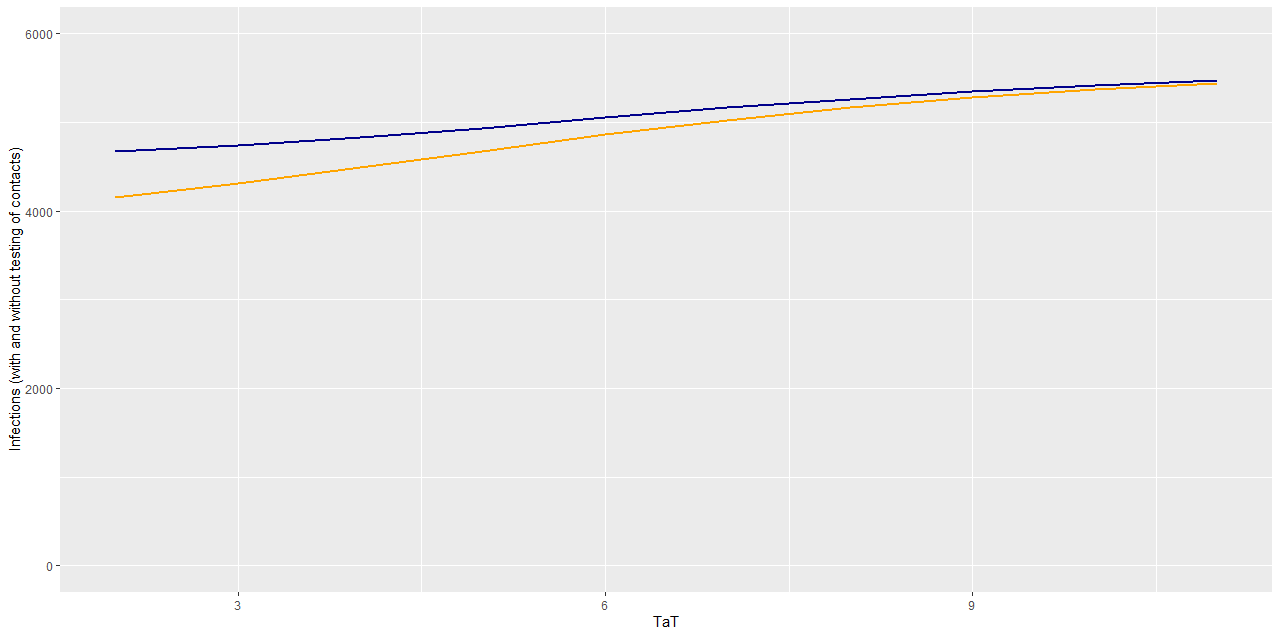
\includegraphics[width=\paperwidth]{line}}
\end{center}
\caption{Difference in mean total infections for CTI versus no CTI with
  different values of TaT}
\label{fig:comparisonByTaT}
\end{figure}

\section{Conclusions}\label{conclusions}

In a structured ABM that simulates key dynamics of Covid-19 transmission and
disease progression, the WHO-recommended strategy of CTI resulted in a
substantial reduction in both the mean number of deaths and the mean number of
total infections. The benefit is greater with shorter TaT times, but remained
substantial even with TaTs of eight days. The difference in mean total
infections between TaTs of 4 and 5 days is more than double that between 9 and
10 days. In our model significant numbers of infections can be averted by
testing the contacts of persons who test positive – a benefit that is greater
with shorter TaTs.

These results suggest that CTI can play a critical role in reducing the size of
outbreaks in the real world and that TaTs should be kept as short as possible in
order to maximise this benefit. Our findings thus broadly confirm those of
Kretzschmar et al and Hellewell et al using a substantially different
methodology.\cite{Kretzschmar2020,Hellewell2020} Apart from the difference in
methodology, our study differs from that of Kretzschmar et al and Hellewell et
al in that we asked whether CTI and different TaT values lead to meaningful
reductions in total infections, while they explored what level of intervention
was needed to reduce the effective reproductive number to below 1. It is
possible that certain levels of intervention would substantially reduce total
infections, but not so much as to bring the effective reproduction number below
1.

Since several of our model parameters are highly uncertain, there is uncertainty
in the model outputs in addition to the already significant stochasticity in the
model. The model outputs should thus at most be considered as illustrative of
underlying epidemiological dynamics rather than as an exact prediction of the
impact of CTI and TaT in the real world.

The model has several limitations. Many of the Covid-19 epidemiological and
disease progression parameters remain highly uncertain. The model does not
account for co-morbidities such as diabetes, HIV and TB. Neither does it account
for movement in and out of the community, a key element of Covid-19 transmission
in the real world. The setting-specific transmission risk parameters in the
structured model were deduced from published literature on TB transmission in a
Cape Town community (No such South African data yet exists for
Covid-19). Finally, we did not attempt to assess the cost-effectiveness of CTI
in this study.

\begin{thebibliography}{1}

\bibitem{Han2020}
  Han, E. et al.
  \newblock Lessons learnt from easing Covid-19 restrictions: an analysis of countries and regions in Asia Pacific and Europe.
  \newblock The Lancet, p. S0140673620320079, 2020.
  \newblock doi: 10.1016/S0140-6736(20)32007-9.

\bibitem{Flaxman2020}
  Flaxman S, Mishra S, Gandy A, et al.
  \newblock Estimating the effects of non-pharmaceutical interventions on
  Covid-19 in Europe.
  \newblock Nature. 2020;584(7820):257-261.
  \newblock doi:10.1038/s41586-020-2405-7

\bibitem{WHO2020}
  World Health Organization
  \newblock Contact Tracing in the Context of Covid-19: Interim Guidance 10 May 2020. Geneva.
  \newblock Available at: https://apps.who.int/iris/rest/bitstreams/1277571/retrieve (Accessed: 26 July 2020).

\bibitem{Fisher2020}
  Fisher, D. and Wilder-Smith, A.
  \newblock The global community needs to swiftly ramp up the response to contain Covid-19.
  \newblock The Lancet, 395(10230), pp. 1109–1110, 2020.
  \newblock doi: 10.1016/S0140-6736(20)30679-6.

\bibitem{Lee2020}
  Lee SW, Yuh WT, Yang JM, et al.
  \newblock Nationwide Results of Covid-19 Contact Tracing in South Korea:
  Individual Participant Data From an Epidemiological Survey.
  \newblock JMIR Med Inform. 2020;8(8):e20992. Published 2020 Aug 25.
  \newblock doi:10.2196/20992

\bibitem{Lee2020b}
  Lee, V. J., Chiew, C. J. and Khong, W. X.
  \newblock Interrupting transmission of Covid-19: lessons from containment efforts in Singapore.
  \newblock Journal of Travel Medicine, 27(3), p. taaa039, 2020.
  \newblock doi: 10.1093/jtm/taaa039.

\bibitem{Kretzschmar2020}
  Kretzschmar, M. E. et al.
  \newblock Impact of delays on effectiveness of contact tracing strategies for Covid-19: a modelling study.
  \newblock The Lancet Public Health, 5(8), pp. e452–e459, 2020.
  \newblock doi: 10.1016/S2468-2667(20)30157-2.

\bibitem{Hellewell2020}
  Hellewell, J. et al.
  \newblock Feasibility of controlling Covid-19 outbreaks by isolation of cases and contacts.
  \newblock The Lancet Global Health, 8(4), pp. e488–e496, 2020.
  \newblock doi: 10.1016/S2214-109X(20)30074-7.

\bibitem{Kwok2019}
  Kwok, K. O. et al.
  \newblock Epidemic Models of Contact Tracing: Systematic Review of Transmission Studies of Severe Acute Respiratory Syndrome and Middle East Respiratory Syndrome.
  \newblock Computational and Structural Biotechnology Journal, 17, pp. 186–194, 2019.
  \newblock doi: 10.1016/j.csbj.2019.01.003.

\bibitem{Andrews2014}
  Andrews, J. R. et al.
  \newblock Integrating Social Contact and Environmental Data in Evaluating Tuberculosis Transmission in a South African Township.
  \newblock The Journal of Infectious Diseases, 210(4), pp. 597–603, 2014.
  \newblock doi: 10.1093/infdis/jiu138.

\bibitem{Vynnycky2010}
  Vynnycky, E. and White, R.
  \newblock An Introduction to Infectious Disease Modelling.
  \newblock OUP Oxford. 2010.

\bibitem{Verity2020}
  Verity, R. et al.
  \newblock Estimates of the severity of coronavirus disease 2019: a model-based analysis.
  \newblock The Lancet Infectious Diseases, 20(6), pp. 669–677, 2020.
  \newblock doi: 10.1016/S1473-3099(20)30243-7.

\bibitem{SACMC2020}
  South African Covid-19 Modelling Consortium.
  \newblock National Covid Epi Model - Updated on 24 July 2020.
  \newblock Available at: https://sacovid19mc.github.io/ (Accessed: 28 July 2020).

\bibitem{Kucirka2020}
  Kucirka, L. M. et al.
  \newblock Variation in False-Negative Rate of Reverse Transcriptase Polymerase Chain Reaction–Based SARS-CoV-2 Tests by Time Since Exposure.
  \newblock Annals of Internal Medicine, pp. M20-1495, 2020.
  \newblock doi: 10.7326/M20-1495.

\bibitem{NICD2020}
  National Institute for Communicable Disease.
  \newblock Covid-19 Testing Summary: South Africa Week 23, 2020.
  \newblock Available at: \url{https://www.nicd.ac.za/wp-content/uploads/2020/06/NICD-COVID-19-Testing-Summary\_-Week-23-2020-005.pdf} (Accessed: 28 July 2020).

\end{thebibliography}

\end{document}
